\documentclass[a4wide]{scrartcl}

\usepackage{a4wide}
\usepackage[top=30pt,bottom=70pt,left=45pt,right=45pt]{geometry}
%\usepackage[margin=60pt]{geometry}
%Sonstiges
\usepackage{nameref}
\makeatletter
\newcommand*{\currentname}{\@currentlabelname}
\makeatother
\usepackage{graphicx}
\usepackage{nameref}

%Header
\usepackage[automark,headsepline]{scrpage2}
\pagestyle{scrheadings}
\ihead{}
\chead{}
\ohead{}
\ifoot{}
\cfoot{\thepage}
\ofoot{}

% References
\usepackage{hyperref}

%Language specific packages
%\usepackage[
%  left=1cm,
%  right=1cm,
%  top=1cm,
%  bottom=1cm,
%  includeheadfoot
%]{geometry}
\usepackage[utf8]{inputenc}
\usepackage[english]{babel}

%Listings
\usepackage{listings}
\usepackage{color}
\definecolor{codegreen}{RGB}{0,128,0}
\definecolor{codegray}{rgb}{0.5,0.5,0.5}
\definecolor{codepurple}{RGB}{175,0,219}
\definecolor{backcolour}{RGB}{241,241,241}
\definecolor{codestring}{RGB}{163,21,21}

\lstdefinestyle{mystyle}{
    language=c++,
    backgroundcolor=\color{backcolour},
    commentstyle=\color{codegreen},
    keywordstyle=\color{codepurple},
    numberstyle=\tiny\color{codegray},
    stringstyle=\color{codestring},
    basicstyle=\footnotesize,
    breakatwhitespace=false,
    breaklines=true,
    captionpos=b,
    keepspaces=true,
    numbers=left,
    numbersep=5pt,
    showspaces=false,
    showstringspaces=false,
    showtabs=false,
    tabsize=2,
}

\lstset{style=mystyle}
%amsPackages
\usepackage{amsmath}
\usepackage{amssymb}

\begin{document}
\title{Google Summer of Code 2018 - Faster Matrix Algebra for ATLAS}
\subtitle{Evaluation Test}
\author{\href{mailto: tellenbach@cip.ifi.lmu.de}{David A. Tellenbach}}
\maketitle
\section{Overview}
\section{Class Design}
The class SymmetricMatrix is actually a class template with two template paramters \texttt{typename Scalar} and \texttt{int Dimension}. The first describes the type of the values of the matrix, the second one its dimension. Since any symmetric matrix is a square matrix specifying one dimension is enough.
\subsection{Storage}
One of the tasks of this evaluation tests was to store only those elements of a symmetric matrix that determines it completely. A $(n \times n)$ matrix contains of $n^2$ elements. In the symmetric case the $ij$-th element is equal to the $ji$-th one, therefore it is sufficient to store
\[
\frac{n(n+1)}{2}    
\]
of its elements, e.g., the upper triangular part of it. Even though matrices are usually considered to be two-dimensional objects hardware memory is linear. The current implementation of the SymmetricMatrix class stores the matrix elements in either an \texttt{std::vector} or \texttt{std::array}. When storing these elements two storage orders can be considered: Row and column major storing.
\begin{description}
    \item[Row Major] The matrix elements are stored packed row by row as illustrated in \autoref{fig1}.
    \begin{figure}
    \centering
        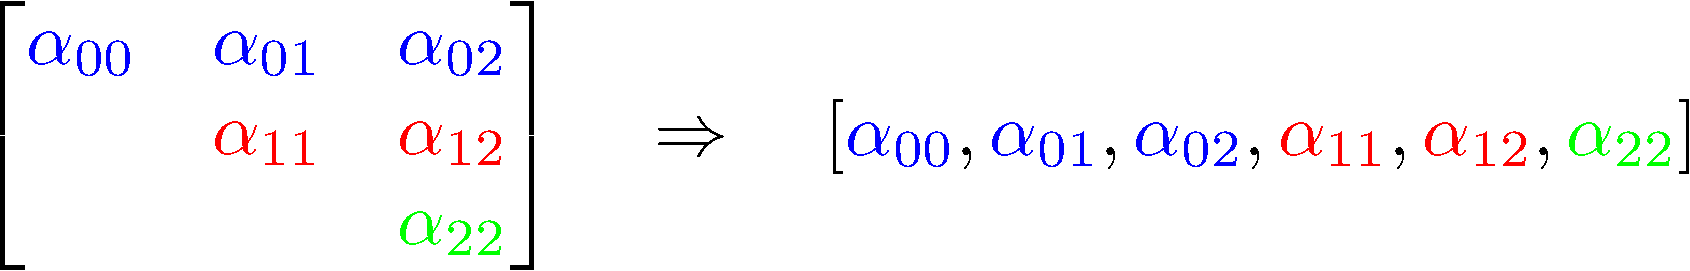
\includegraphics[scale=0.35]{img/RowMajor.pdf}
        \caption{Packed storage of a $3 \times 3$ matrix in row major order.}
        \label{fig1}
    \end{figure}
    Currently the SymmetricMatrix class stores matrix elements row major.
    \item[Column Major] The other storage order that can be considered is to store matrix elements packed column by column. Such a storage order is called column major and is illustrated in \autoref{fig2}.
    \begin{figure}
    \centering
        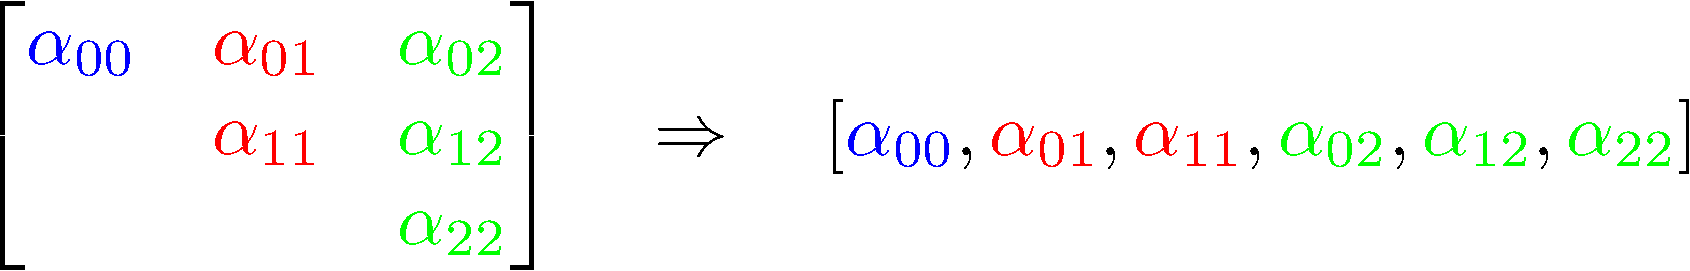
\includegraphics[scale=0.35]{img/ColumnMajor.pdf}
        \caption{Packed storage of a $3 \times 3$ matrix in column major order.}
        \label{fig2}
    \end{figure}
\end{description}
Storage order can dramatically determine the performance of matrix operations since it determines who matrix elements are loaded into cache. 
\subsection{Compile- and runtime}
Following the design of Eigen the implementation of this evaluation test contains both fixed and dynamically sized symmetric matrices. The generic class template \texttt{SymmetricMatrix<typename Scalar, int Dimension>} contains the implementation of fixed sized matrices. The elements are stored in an \texttt{std::array}. The size of this underlying container is calculated at compile-time. \newline
If the special dimension \texttt{Eigen::Dimension} that is just a typedef for $-1$ is passed, the partial template specialization \texttt{SymmetricMatrix<typename Scalar, Eigen::Dynamic>} is used. This class is more flexible than the fixed sized case but is less performant as \autoref{tbl1} shows.\newline\newline
\begin{table}
\centering
\begin{tabular}{r|r|r}
Dimension & t1 (Fixed)  & t2 (Dynamic)  \\ \hline \hline
$10$  & $215$~ns & $731$~ns \\
$20$  & $656$~ns & $2306$~ns \\
$30$  & $1413$~ns & $4573$~ns \\
$40$  & $2530$~ns & $7844$~ns \\
$50$  & $3914$~ns & $11896$~ns \\
$60$  & $5812$~ns & $17107$~ns \\
$70$  & $7723$~ns & $23577$~ns \\
$80$  & $10185$~ns & $30322$~ns \\
$90$  & $13629$~ns & $39718$~ns \\
$100$ & $16239$~ns & $47402$~ns
\end{tabular}
\caption{Time consumption of adding fixed sized and dynamically sized matrices.}
\label{tbl1}
\end{table}
Since the memory allocation for fixed sized matrices is done during compilation it is completly located on the stack. Since stack size is limited matrices of this type are limited to relativly small dimensions. Large matrices containing tousands of elements should (and often must) be allocated on the heap. In this case dynamically sized matrices are the right choice.
\subsection{Addition and Subtraction}
Addition and subtraction are important component wise operations of matrices its complexity is always bounded from above by $n^2$ for a matrix of dimension $n$. Since we are not storing all $n^2$ elements of a symmetric matrix, we can perform even better.\newline
The actual implementation works just by adding up the elements of the underlying containers, i.e., instances of \texttt{std::array} in the fixed sized case and \texttt{std::vector} in the dynamically sized case. E.g., \autoref{lst1} show the implementation of the addition of two dynamically sized matrices.
\begin{table}
\begin{lstlisting}[caption={Overloaded operator $+$ for the addition of two dynamically sized matrices.},label=lst1]
SymmetricMatrix<Scalar>
operator+(const SymmetricMatrix<Scalar>& other) {
    // Check if both dynamic dimensions match
    if (dimension != other.dim()) {
        throw std::invalid_argument("Operation + cannot be performed "
                                    "for instances of SymmetricMatrix "
                                    "with not matching dimension");
        }

    // Construct new matrix and set underlying std::vector 
    // by passing the underlying std::vector of this
    SymmetricMatrix<Scalar> ret(elements);      

    // Just add up both underlying std::vector
    for (int i = 0; i < elements.size(); ++i) {
        ret.elements[i] += other.elements[i];
    }
    return ret;
}
\end{lstlisting}
\end{table}
\subsection{Multiplication}
Multiplication is a far more complex task than simple component wise operations like addition or subtraction. The simple implementation contains of three nested for-loops and the constant switch between matrix rows and matrix columns is pure cache horror. Big projects like BLAS have optimized matrix multiplication and its implementations like the Intel Math Kernel Library are complex and not easy to mimic. Trying to create an implementation beating or even being competitive with Eigens internal multiplication implementation is no realistic task for this evaluation test.\newline
However the product of two symmetric matrices is in general not symmetric (it is and only is if the matrix product is commutative). Therefore this implementation uses the following trick: We construct instances of Eigen::Matrix from the symmetric matrices and use Eigens internal mechanism to multiply these. Since the result of the multiplication will be Eigen::Matrix anyway, we won't have to issue about memory usage.\newline
One could now argue that the temporary constructed instances of Eigen::Matrix will consume memory. This is right in general but by using an optimization technique that can be avoided (at least when the compiler runs with optimizer flags). See \autoref{lst2} to see a concrete implementation of the multiplication of the symmetric matrices of dynamic size.
\begin{table}
\begin{lstlisting}[caption={Overloaded operator $*$ for the multiplication of two dynamically sized matrices.},label=lst2]
Eigen::Matrix<Scalar, Eigen::Dynamic, Eigen::Dynamic>
operator*(SymmetricMatrix<Scalar>& other) {
    // The instance of Eigen::Matrix is constructed in return statement
    // This allow the compiler to optimize temporary instances away
    return Eigen::Matrix<Scalar, Eigen::Dynamic, Eigen::Dynamic>(
               constructEigenMatrix() * other.constructEigenMatrix()
           );
}
\end{lstlisting}
\end{table}
\subsection{Runtime Exceptions and Compiletime Errors}
Another task of the evaluation test was to throw exceptions whenever an operations is performed where the dimensions of the operands don't match. In the particular case one has to consider the both cases of dynamically and fixed sized matrices differently:\newline
\begin{description}
\item[Fixed size operates with fixed size] The easiest case. The compiler performs statically typechecks and the implementation guarantees that a compile time error will raise if the operands have non-matching dimensions. This holds for operations with fixed sized instances of SymmetricMatrix and fixed sized instances of Eigen::Matrix. See \autoref{lst3} for an example that will not compile.
\item[Fixed size operates with dynamic size] In these cases the implementation checks if the dimensions match during runtime. If they dont, an excpetion is thrown.
\item[Dynamic size operates with dynamic size] In these cases the implementation checks if the dimensions match during runtime. If they dont, an excpetion is thrown. See \autoref{lst4} for an try-catch example.
\end{description}
\begin{table}
\begin{lstlisting}[caption={Addition of matrices with different fixed size. This example will not compile.},label=lst3]
// Symmetric matrix of ints with fixed dimension 3 filled with random values
SymmetricMatrix<int, 3> mat1 = SymmetricMatrix<int, 3>::Random();

// Symmetric matrix of ints with fixed dimension 5 filled with random values
SymmetricMatrix<int, 5> mat2 = SymmetricMatrix<int, 5>::Random();

mat1 + mat2;    // Compiler error
\end{lstlisting}
\end{table}
\begin{table}
\begin{lstlisting}[caption={Addition of matrices with different dynamic size.},label=lst4]
// Symmetric matrix of ints with dynamic dimension 3 filled with random values
SymmetricMatrix<int> mat1 = SymmetricMatrix<int>::Random(3);

// Symmetric matrix of ints with dynamic dimension 5 filled with random values
SymmetricMatrix<int, 5> mat2 = SymmetricMatrix<int>::Random(5);

try {
    mat1 + mat2;
} catch (std::exception& ex) {
    std::cout << ex.what() << "\n";     
}
/* Output: Operation + cannot be performed for instances of SymmetricMatrix with not matching dimension */
\end{lstlisting}
\end{table}
\section{Benchmarks}
\section{Futur Work}
This section explains 
\subsection{Existing matrix classes in Eigen}
\subsection{Implementation ideas}
\end{document}












